
\documentclass[a4paper,11pt]{article}
\usepackage[a4paper, margin=8em]{geometry}

% usa i pacchetti per la scrittura in italiano
\usepackage[french,italian]{babel}
\usepackage[T1]{fontenc}
\usepackage[utf8]{inputenc}
\frenchspacing 

% usa i pacchetti per la formattazione matematica
\usepackage{amsmath, amssymb, amsthm, amsfonts}

% usa altri pacchetti
\usepackage{gensymb}
\usepackage{hyperref}
\usepackage{standalone}

\usepackage{colortbl}

\usepackage{xstring}
\usepackage{karnaugh-map}

% imposta il titolo
\title{Electronics for Embedded Systems notes}
\author{Luca Seggiani}
\date{2026}

% spaziatura liste
\usepackage{enumitem}
\setlist[itemize]{noitemsep, topsep=4pt, partopsep=0pt, parsep=2pt, leftmargin=*}
\setlist[enumerate]{noitemsep, topsep=4pt, partopsep=0pt, parsep=2pt, leftmargin=*}

% imposta lo stile
% usa helvetica
\usepackage[scaled]{helvet}
% usa palatino
\usepackage{palatino}
% usa un font monospazio guardabile
\usepackage{lmodern}

\renewcommand{\rmdefault}{ppl}
\renewcommand{\sfdefault}{phv}
\renewcommand{\ttdefault}{lmtt}

% circuiti
\usepackage{circuitikz}
\usetikzlibrary{babel}

% testo cerchiato
\newcommand*\circled[1]{\tikz[baseline=(char.base)]{
            \node[shape=circle,draw,inner sep=2pt] (char) {#1};}}

% disponi il titolo
\makeatletter
\renewcommand{\maketitle} {
	\begin{center} 
		\begin{minipage}[t]{.8\textwidth}
			\textsf{\huge\bfseries \@title} 
		\end{minipage}%
		\begin{minipage}[t]{.2\textwidth}
			\raggedleft \vspace{-1.65em}
			\textsf{\small \@author} \vfill
			\textsf{\small \@date}
		\end{minipage}
		\par
	\end{center}

	\thispagestyle{empty}
	\pagestyle{fancy}
}
\makeatother

% disponi teoremi
\usepackage{tcolorbox}
\newtcolorbox[auto counter, number within=section]{theorem}[2][]{%
	colback=blue!10, 
	colframe=blue!40!black, 
	sharp corners=northwest,
	fonttitle=\sffamily\bfseries, 
	title=Theorem~\thetcbcounter: #2, 
	#1
}

% disponi definizioni
\newtcolorbox[auto counter, number within=section]{definition}[2][]{%
	colback=red!10,
	colframe=red!40!black,
	sharp corners=northwest,
	fonttitle=\sffamily\bfseries,
	title=Definition~\thetcbcounter: #2,
	#1
}

% disponi codice
\usepackage{listings}
\usepackage[table]{xcolor}

\definecolor{codegreen}{rgb}{0,0.6,0}
\definecolor{codegray}{rgb}{0.5,0.5,0.5}
\definecolor{codepurple}{rgb}{0.58,0,0.82}
\definecolor{backcolour}{rgb}{0.95,0.95,0.92}

\lstdefinestyle{codestyle}{
		backgroundcolor=\color{black!5}, 
		commentstyle=\color{codegreen},
		keywordstyle=\bfseries\color{magenta},
		numberstyle=\sffamily\tiny\color{black!60},
		stringstyle=\color{green!50!black},
		basicstyle=\ttfamily\footnotesize,
		breakatwhitespace=false,         
		breaklines=true,                 
		captionpos=b,                    
		keepspaces=true,                 
		numbers=left,                    
		numbersep=5pt,                  
		showspaces=false,                
		showstringspaces=false,
		showtabs=false,                  
		tabsize=2
}

\lstdefinestyle{shellstyle}{
		backgroundcolor=\color{black!5}, 
		basicstyle=\ttfamily\footnotesize\color{black}, 
		commentstyle=\color{black}, 
		keywordstyle=\color{black},
		numberstyle=\color{black!5},
		stringstyle=\color{black}, 
		showspaces=false,
		showstringspaces=false, 
		showtabs=false, 
		tabsize=2, 
		numbers=none, 
		breaklines=true
}

\lstdefinelanguage{x86}{ 
  keywords={AAA, AAD, AAM, AAS, ADC, ADCB, ADCW, ADCL, ADD, ADDB, ADDW, ADDL, AND, ANDB, ANDW, ANDL,
        ARPL, BOUND, BSF, BSFL, BSFW, BSR, BSRL, BSRW, BSWAP, BT, BTC, BTCB, BTCW, BTCL, BTR, 
        BTRB, BTRW, BTRL, BTS, BTSB, BTSW, BTSL, CALL, CBW, CDQ, CLC, CLD, CLI, CLTS, CMC, CMP,
        CMPB, CMPW, CMPL, CMPS, CMPSB, CMPSD, CMPSW, CMPXCHG, CMPXCHGB, CMPXCHGW, CMPXCHGL,
        CMPXCHG8B, CPUID, CWDE, DAA, DAS, DEC, DECB, DECW, DECL, DIV, DIVB, DIVW, DIVL, ENTER,
        HLT, IDIV, IDIVB, IDIVW, IDIVL, IMUL, IMULB, IMULW, IMULL, IN, INB, INW, INL, INC, INCB,
        INCW, INCL, INS, INSB, INSD, INSW, INT, INT3, INTO, INVD, INVLPG, IRET, IRETD, JA, JAE,
        JB, JBE, JC, JCXZ, JE, JECXZ, JG, JGE, JL, JLE, JMP, JNA, JNAE, JNB, JNBE, JNC, JNE, JNG,
        JNGE, JNL, JNLE, JNO, JNP, JNS, JNZ, JO, JP, JPE, JPO, JS, JZ, LAHF, LAR, LCALL, LDS,
        LEA, LEAVE, LES, LFS, LGDT, LGS, LIDT, LMSW, LOCK, LODSB, LODSD, LODSW, LOOP, LOOPE,
        LOOPNE, LSL, LSS, LTR, MOV, MOVB, MOVW, MOVL, MOVSB, MOVSD, MOVSW, MOVSX, MOVSXB,
        MOVSXW, MOVSXL, MOVZX, MOVZXB, MOVZXW, MOVZXL, MUL, MULB, MULW, MULL, NEG, NEGB, NEGW,
        NEGL, NOP, NOT, NOTB, NOTW, NOTL, OR, ORB, ORW, ORL, OUT, OUTB, OUTW, OUTL, OUTSB, OUTSD,
        OUTSW, POP, POPL, POPW, POPB, POPA, POPAD, POPF, POPFD, PUSH, PUSHL, PUSHW, PUSHB, PUSHA, 
        RCLL, RCR, RCRB, RCRW, RCRL, RDMSR, RDPMC, RDTSC, REP, REPE, REPNE, RET, ROL, ROLB, ROLW,
        ROLL, ROR, RORB, RORW, RORL, SAHF, SAL, SALB, SALW, SALL, SAR, SARB, SARW, SARL, SBB,
        SBBB, SBBW, SBBL, SCASB, SCASD, SCASW, SETA, SETAE, SETB, SETBE, SETC, SETE, SETG, SETGE,
        SETL, SETLE, SETNA, SETNAE, SETNB, SETNBE, SETNC, SETNE, SETNG, SETNGE, SETNL, SETNLE,
        SETNO, SETNP, SETNS, SETNZ, SETO, SETP, SETPE, SETPO, SETS, SETZ, SGDT, SHL, SHLB, SHLW,
        SHLL, SHLD, SHR, SHRB, SHRW, SHRL, SHRD, SIDT, SLDT, SMSW, STC, STD, STI, STOSB, STOSD,
        STOSW, STR, SUB, SUBB, SUBW, SUBL, TEST, TESTB, TESTW, TESTL, VERR, VERW, WAIT, WBINVD,
        XADD, XADDB, XADDW, XADDL, XCHG, XCHGB, XCHGW, XCHGL, XLAT, XLATB, XOR, XORB, XORW, XORL},
  keywordstyle=\color{blue}\bfseries,
  ndkeywordstyle=\color{darkgray}\bfseries,
  identifierstyle=\color{black},
  sensitive=false,
  comment=[l]{\#},
  morecomment=[s]{/*}{*/},
  commentstyle=\color{purple}\ttfamily,
  stringstyle=\color{red}\ttfamily,
  morestring=[b]',
  morestring=[b]"
}

\lstdefinelanguage{riscv}{
  keywords={
    LUI, AUIPC,
    JAL, JALR,
    BEQ, BNE, BLT, BGE, BLTU, BGEU,
    LB, LH, LW, LBU, LHU, LD,
    SB, SH, SW, SD,
    ADDI, SLTI, SLTIU, XORI, ORI, ANDI,
    SLLI, SRLI, SRAI,
    ADD, SUB, SLL, SLT, SLTU, XOR, SRL, SRA, OR, AND,
    ADDIW, SLLIW, SRLIW, SRAIW,
    ADDW, SUBW, SLLW, SRLW, SRAW,
    MUL, MULH, MULHSU, MULHU, DIV, DIVU, REM, REMU,
    MULW, DIVW, DIVUW, REMW, REMUW,
    LR.W, SC.W, AMOSWAP.W, AMOADD.W, AMOXOR.W,
    AMOAND.W, AMOOR.W, AMOMIN.W, AMOMAX.W,
    AMOMINU.W, AMOMAXU.W,
    LR.D, SC.D, AMOSWAP.D, AMOADD.D, AMOXOR.D,
    AMOAND.D, AMOOR.D, AMOMIN.D, AMOMAX.D,
    AMOMINU.D, AMOMAXU.D,
    FLW, FSW,
    FMADD.S, FMSUB.S, FNMSUB.S, FNMADD.S,
    FADD.S, FSUB.S, FMUL.S, FDIV.S, FSQRT.S,
    FSGNJ.S, FSGNJN.S, FSGNJX.S,
    FMIN.S, FMAX.S,
    FCVT.W.S, FCVT.WU.S, FCVT.S.W, FCVT.S.WU,
    FMV.X.W, FMV.W.X,
    FEQ.S, FLT.S, FLE.S,
    FLD, FSD,
    FMADD.D, FMSUB.D, FNMSUB.D, FNMADD.D,
    FADD.D, FSUB.D, FMUL.D, FDIV.D, FSQRT.D,
    FSGNJ.D, FSGNJN.D, FSGNJX.D,
    FMIN.D, FMAX.D,
    FCVT.W.D, FCVT.WU.D, FCVT.D.W, FCVT.D.WU,
    FCVT.S.D, FCVT.D.S,
    FMV.X.D, FMV.D.X,
    FEQ.D, FLT.D, FLE.D,
    CSRRW, CSRRS, CSRRC,
    CSRRWI, CSRRSI, CSRRCI,
    FENCE.I,
    FENCE,
    ECALL, EBREAK,
    MRET, SRET, URET,
    WFI,
    SFENCE.VMA,
    NOP, LI, LA, MV,
    NOT, NEG, NEGW,
    SEQZ, SNEZ, SLTZ, SGTZ,
    BEQZ, BNEZ, BLEZ, BGEZ, BLTZ, BGTZ,
    BGT, BLE, BGTU, BLEU,
    J, JR, RET,
    CALL, TAIL,
    RDINSTRET, RDCYCLE, RDTIME,
    CSRR, CSRW, CSRS, CSRC,
    CSRWI, CSRSI, CSRCI
  },
  keywordstyle=\color{blue}\bfseries,
  ndkeywordstyle=\color{darkgray}\bfseries,
  identifierstyle=\color{black},
  sensitive=false,
  comment=[l]{\#},
  morecomment=[s]{/*}{*/},
  commentstyle=\color{purple}\ttfamily,
  stringstyle=\color{red}\ttfamily,
  morestring=[b]',
  morestring=[b]"
}

\lstdefinelanguage{arm}{
  keywords={
    ADC, ADD, AND, BIC, CMN, CMP, EOR, MOV, MVN,
    RSB, RSC, SBC, SUB, TST, TEQ,
    MLA, MLS, MUL, SMLAL, SMULL, UMLAL, UMULL,
    QADD, QSUB, QDADD, QDSUB,
    QADD16, QADD8, QASX, QSAX,
    QSUB16, QSUB8, QSAX, QSUBADDX,
    ASR, LSL, LSR, ROR, RRX,
    B, BL, BX, BLX,
    BXJ,
    BEQ, BNE, BCS, BHS, BCC, BLO,
    BMI, BPL, BVS, BVC,
    BHI, BLS, BGE, BLT, BGT, BLE,
    BAL,
    LDR, LDRB, LDRH, LDRSB, LDRSH,
    LDRD, LDM, LDMIA, LDMIB, LDMDA, LDMDB,
    LDRT, LDRBT, LDRHT, LDRSBT, LDRSHT,
    STR, STRB, STRH, STRD,
    STM, STMIA, STMIB, STMDA, STMDB,
    STRT, STRBT, STRHT,
    PUSH, POP,
    SWP, SWPB,
    REV, REV16, REVSH,
    BFC, BFI, BFXIL, SBFX, UBFX,
    CLZ,
    LDREX, LDREXB, LDREXH, LDREXD,
    STREX, STREXB, STREXH, STREXD,
    DMB, DSB, ISB,
    MCR, MCRR, MRC, MRRC,
    MRS, MSR,
    CPS, SETEND, SVC, BKPT,
    CLREX, WFE, WFI, SEV,
    YIELD, NOP,
    VLDR, VSTR,
    VMOV, VABS, VNEG,
    VADD, VSUB, VMUL, VDIV,
    VMLA, VMLS, VNMLA, VNMLS, VNMUL,
    VMAX, VMIN,
    VSQRT,
    VCMP, VCMPE,
    VCVT,
    VCLZ, VCLS,
    VAND, VORR, VEOR, VBIC, VMVN,
    VLD1, VLD2, VLD3, VLD4,
    VST1, VST2, VST3, VST4,
    ADR, ADCS, ADDS, SUBS, MOVS, ANDS, ORRS, EORS
  },
  keywordstyle=\color{blue}\bfseries,
  ndkeywordstyle=\color{darkgray}\bfseries,
  identifierstyle=\color{black},
  sensitive=false,
  comment=[l]{@},
  morecomment=[l]{;},
  morecomment=[s]{/*}{*/},
  commentstyle=\color{purple}\ttfamily,
  stringstyle=\color{red}\ttfamily,
  morestring=[b]',
  morestring=[b]"
}

\lstset{style=codestyle, language=C}

% disponi sezioni
\usepackage{titlesec}

\titleformat{\section}
	{\sffamily\Large\bfseries} 
	{\thesection}{1em}{} 
\titleformat{\subsection}
	{\sffamily\large\bfseries}   
	{\thesubsection}{1em}{} 
\titleformat{\subsubsection}
	{\sffamily\normalsize\bfseries} 
	{\thesubsubsection}{1em}{}

% tikz
\usepackage{tikz}

% float
\usepackage{float}

% grafici
\usepackage{pgfplots}
\pgfplotsset{width=10cm,compat=1.9}

% disponi alberi
\usepackage{forest}

\forestset{
	rectstyle/.style={
		for tree={rectangle,draw,font=\large\sffamily}
	},
	roundstyle/.style={
		for tree={circle,draw,font=\large}
	}
}

% disponi algoritmi
\usepackage{algorithm}
\usepackage{algorithmic}
\makeatletter
\renewcommand{\ALG@name}{Algorithm}
\makeatother

% disponi numeri di pagina
\usepackage{fancyhdr}
\fancyhf{} 
\fancyfoot[L]{\sffamily{\thepage}}

\makeatletter
\fancyhead[L]{\raisebox{1ex}[0pt][0pt]{\sffamily{\@title \ \@date}}} 
\fancyhead[R]{\raisebox{1ex}[0pt][0pt]{\sffamily{\@author}}}
\makeatother

\begin{document}
% sezione (data)
\section{Lesson 14-10-26}

% stili pagina
\thispagestyle{empty}
\pagestyle{fancy}

% testo
In the last lesson we started cache memories.

\subsubsection{Cache parameters}

Let's first look at some \textit{parameters} regarding cachelines and DRAM blocks.

\begin{center}
	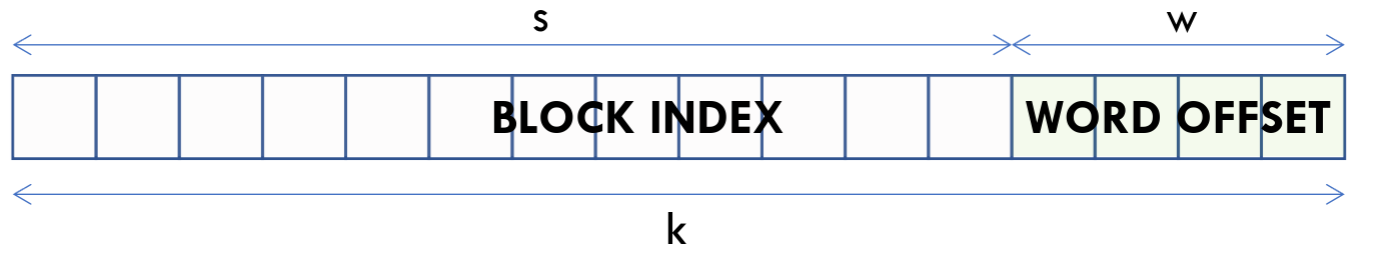
\includegraphics[scale=0.22]{../figures/cache_params.png}
\end{center}

From the figure we see how a standard address is divided in multiple regions, that is:
\begin{itemize}
	\item The \textbf{block index}, of width $s$, which identifies the block the address pertains to;
	\item The \textbf{word offset}, of width $w$, which identifies a single word in the block (shared by multiple words).
\end{itemize}

The parameters ($s$ and $w$, as well as the full address size $k$) are defined below.

\begin{itemize}
\item
\textbf{Mainsize}: the size of DRAM main memory (in words). We have:
$$
k = \log_2 ( \text{Mainsize} ) 
$$
\item
\textbf{Cachesize}: the size of SRAM (in words);
\item
\textbf{Linesize}: the number of words in a cache line. We have:
$$
w = \log_2 ( \text{Linesize} )
$$
\item
\textbf{Nlines}: the number of cache lines. It's defined as:
$$
\text{Nlines} = \frac{\text{Cachesize}}{\text{Linesize}} 
$$
We also define:
$$
r = \log_2 ( \text{Nlines} )
$$
\item
\textbf{Nblocks}: the number of blocks in DRAM. It's defined as:
$$
\text{Nblocks} = \text{Mainsize}{Linesize}
$$
We also define:
$$
s = \log_2 ( \text{Nblocks} )
$$
\end{itemize}

\subsubsection{CAM cache}

The first approach introduced involved a CAM.
Let's give a quick demonstration. 

\begin{center}
	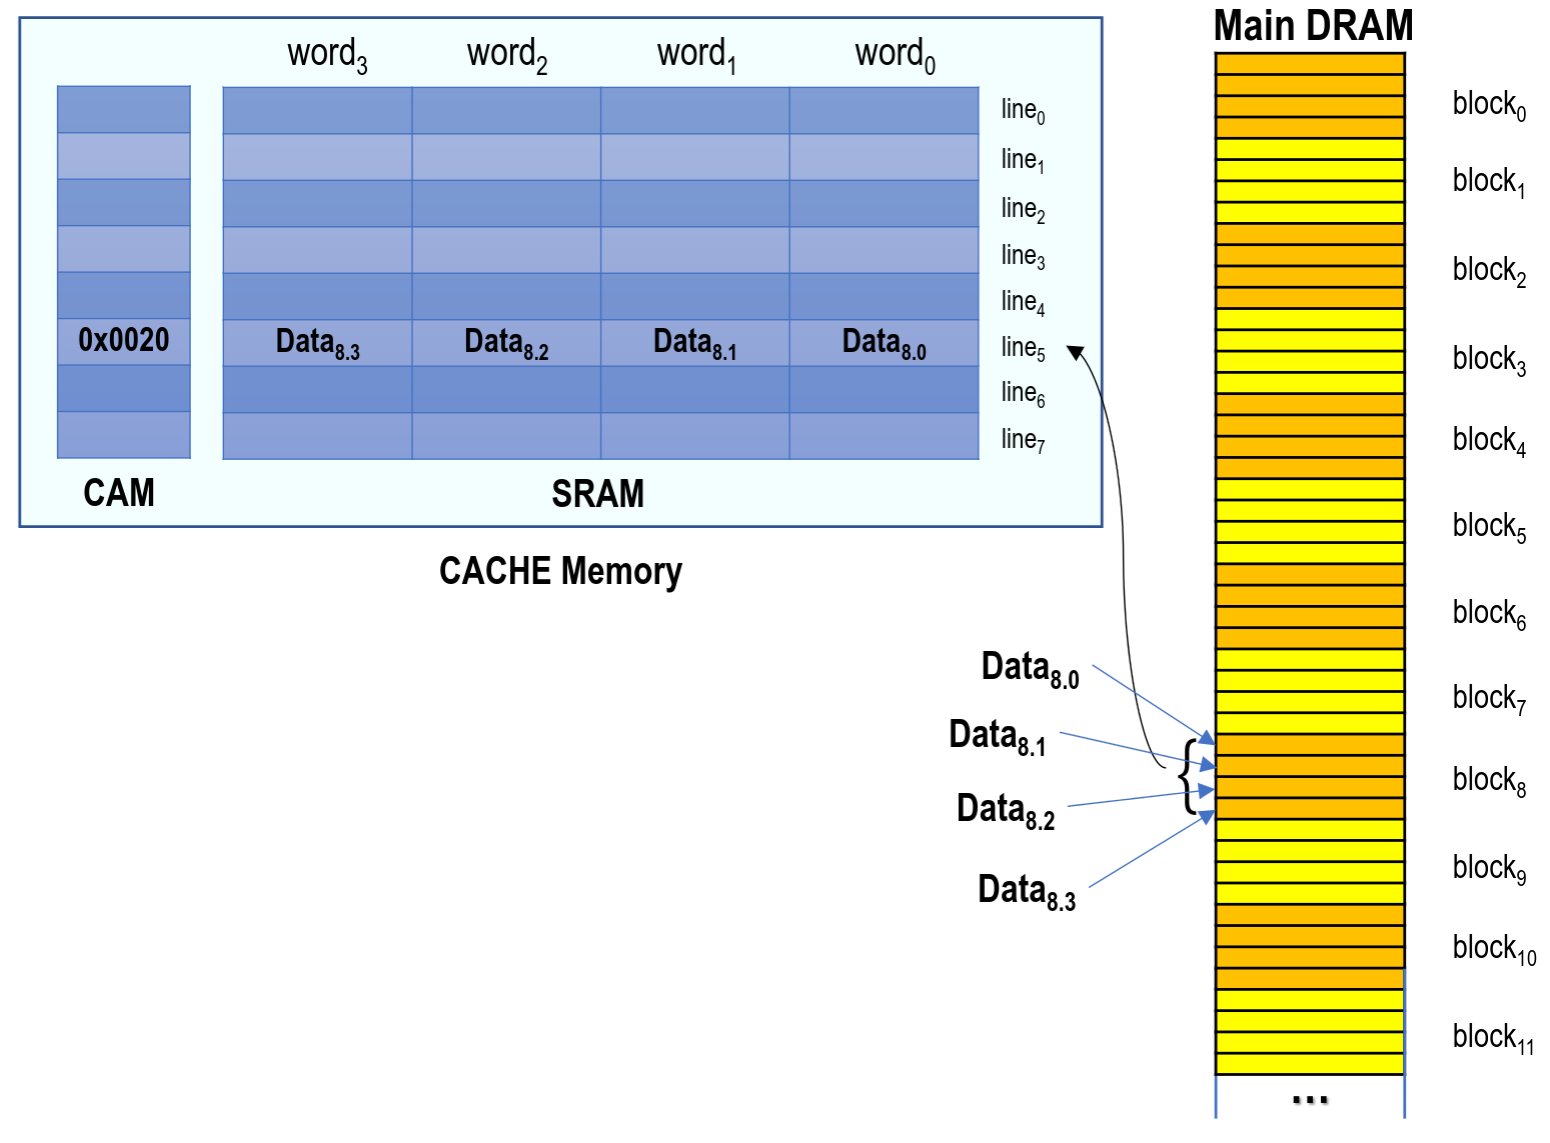
\includegraphics[scale=0.22]{../figures/cam_cache.png}
\end{center}

\begin{itemize}
	\item 
Say the cache line is 4 words large, with the whole cache initially empty.
The processor issues a read for the word at address \texttt{0x0022} (the Read Address). 
This belongs to the ninth block (block8), and the block address is \texttt{0x0020} (the Block Address). 
Say we mean to store block8 in the sixth cache line (line5): to do this we store its address in the sixth location of the CAM.
After this is done, we return word2 from the cache line.

	\item
		Next, assume the processor issues a read for the word at address \texttt{0x0023} (the Read Address). This belongs to the ninth block (block8), as well, so when we match the Block Address \texttt{0x0020} to the CAM, we get a HIT, and the CAM returns the line5.
At this point we can quickly read word3 from the cache line
\end{itemize}

There are some clear \textit{policies} to define for this:
\begin{itemize}
	\item 
When reading from DRAM and storing in cache, we must decide where to write the data.
This is the \textbf{mapping} policy;
\item 
If the cache is full and new data has to be written, some previous data must be erased.
This is the \textbf{replacement} policy;
\item 
When writing some data, cache and main memory should be both updated.
this is the \textbf{consistency} policy.

\end{itemize}

\subsubsection{Direct mapping cache}

An alternative approach is one where the association between a block in main memory and a cache line is unique by design.
Such an unique mapping, in hardware, is easily implemented via a modulo hash operation, by taking the least significant $r$ bits of the block index as a line index, and the most significant bits as a unique tag.

\begin{center}
	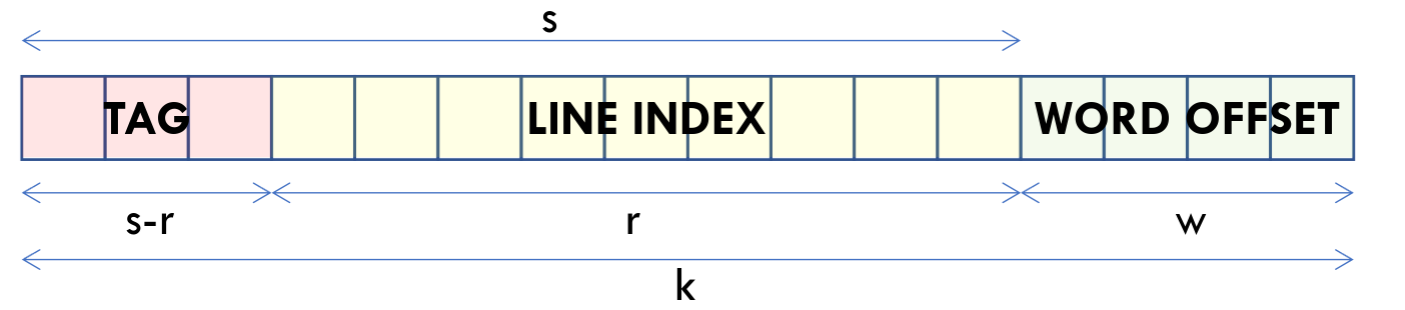
\includegraphics[scale=0.22]{../figures/cache_good.png}
\end{center}

In practice, we don't need to compute anything, as the index can be directly obtained
from the address word by proper masking and/or shifting:
$$
\text{Line} = (\text{Address} >> 2) \% (\text{Nlines} - 1) 
$$
in binary, where $(\text{Address} >> 2)$ is nothing more than the \textit{Block Address}.

Multiple blocks are assigned to the same cache line (as we said, the DRAM is bigger than the whole SRAM), with only $\frac{\text{Nblocks}}{\text{Nlines}}$ blocks mapped to each cache line.
Only one of them is loaded in cache at any given time (so we have to \textit{evict} old ones).

Consider blocks in main memory mapped to the same cache line.
\begin{itemize}
	\item 
	The address of each block always has the $w$ least significant bits at 0, so we do not need to store this information in the CAM.
	\item
	The \textit{Line} index is the same for all blocks assigned to the same cache line, as it corresponds to the cache line to which they are mapped, so we also do not need to store this information in the CAM.
\end{itemize}

Only the \textit{TAG}s differ: the TAG is made of the upper $s - r$ bits of the address.
This is the only information that needs to be stored in the CAM:
different blocks mapped to the same
cache line are guaranteed to have
different TAG.

\begin{center}
	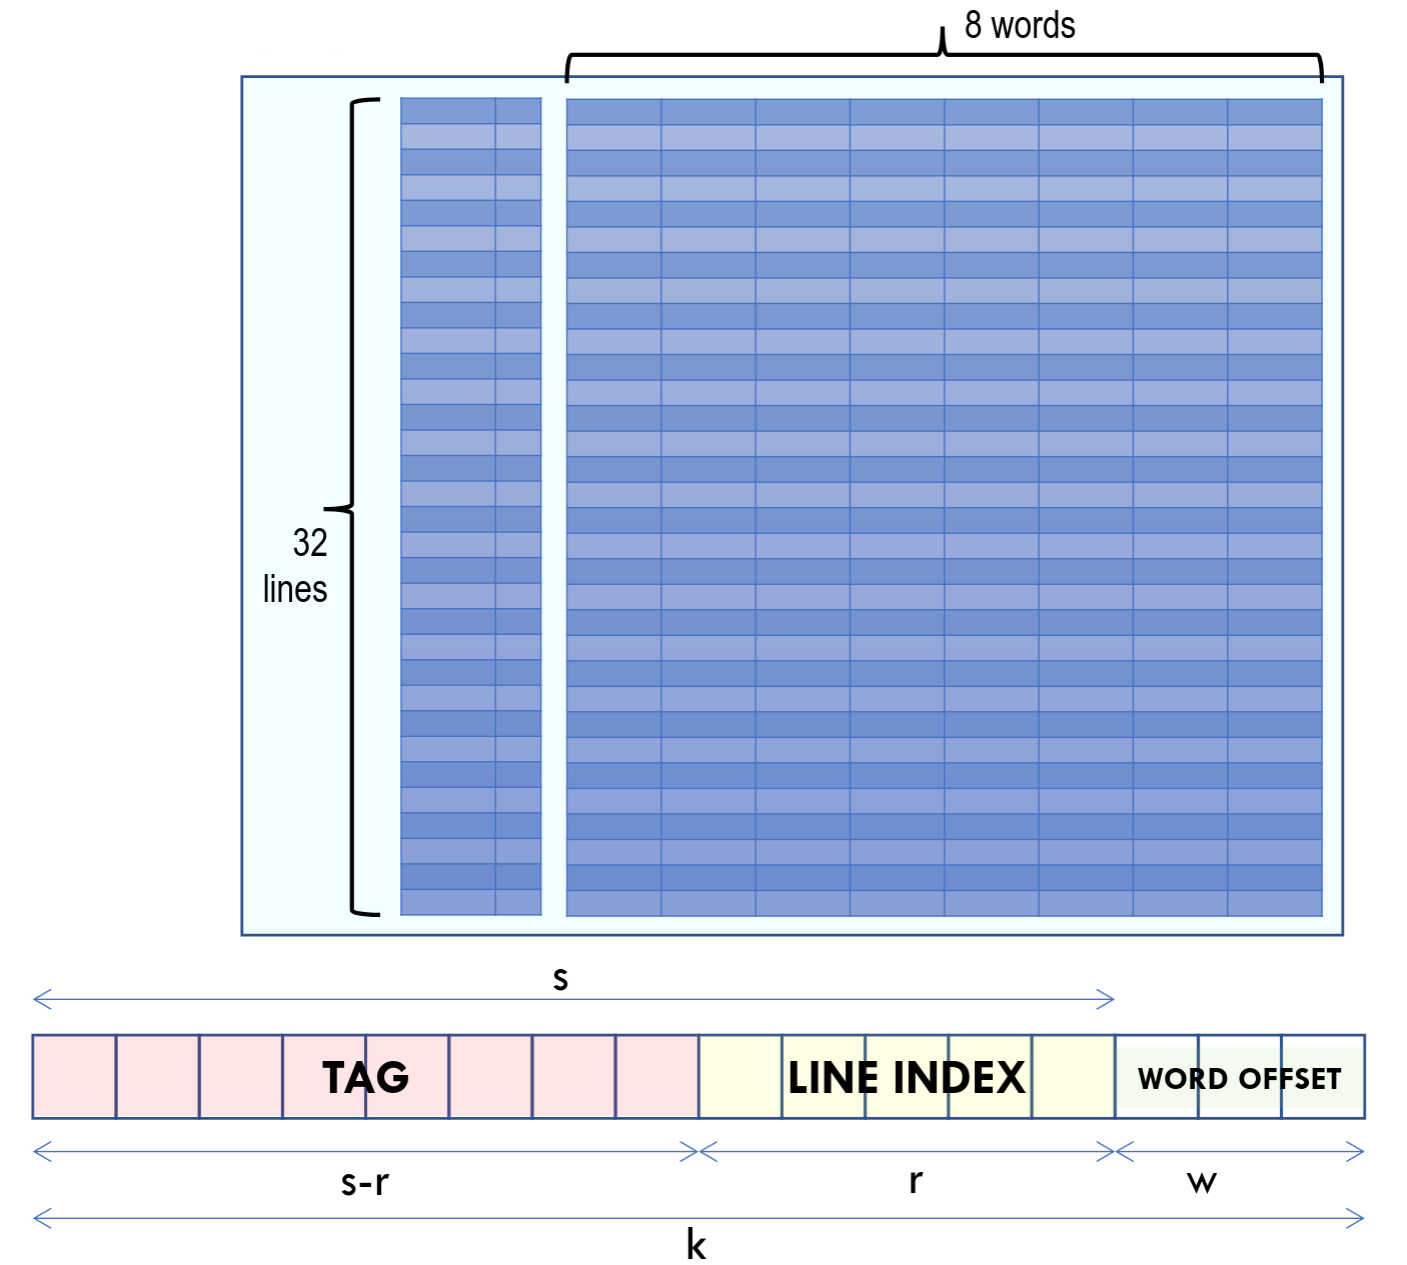
\includegraphics[scale=0.22]{../figures/cache_direct_cam.png}
\end{center}

At this point, given the address of some data, what we need to do is:
\begin{itemize}
	\item Match the TAG with the CAM at location pointed by \textit{Line} index (only if the entry is valid).
		The CAM is actually made of \textit{Nlines} separate CAMs of a single word;
	\item 
On MISS, we read the memory block from DRAM at address \textit{Blockaddress}. 
The TAG is stored in the CAM, in the location pointed by \textit{Lineindex}, so we can instantly match (and rewrite for misses). The block data is stored in the SRAM, in the line pointed by the \textit{Line} index, possibly replacing other data already present.
Then, a validity bit is set for the line, and we can read the word at \textit{Word Offset} in the line pointed by the \textit{Line} index.

A word can be spent on the validity bit: this is concatenated to the TAG, and when we match we match TAGs with the validity bit at 1. If the cacheline was never written to then the validity bit is at 0 and we definitely don't match;
	\item 
On HIT, we just read the word at \textit{Word Offset} in the line pointed by the \textit{Line} index. 
\end{itemize}

Let's look at the \textit{performance} of this.
The advantages are that direct mapping cache is very simple to implement, cheap.
We don’t even need a CAM, as the \textit{Line} index already points to the only location to match.
This makes for low power consumption, and the simplest replacement policy: no policy at all, since it's built into the memory structure.

The disadvantages are that we may replace some data even if the cache is not full (on misses), leading to poorer performance. The HIT Rate is also the poorest out of all cache designs we'll see.

\subsubsection{Fully associative mapping cache}

This is the one we introduced in 9.2.4.
No pre-determined association is defined between a main memory block and a line: when loaded from DRAM, a block is stored in the first available cache line.
This means that there is no pre-determined \textit{Line} index. 

\begin{center}
	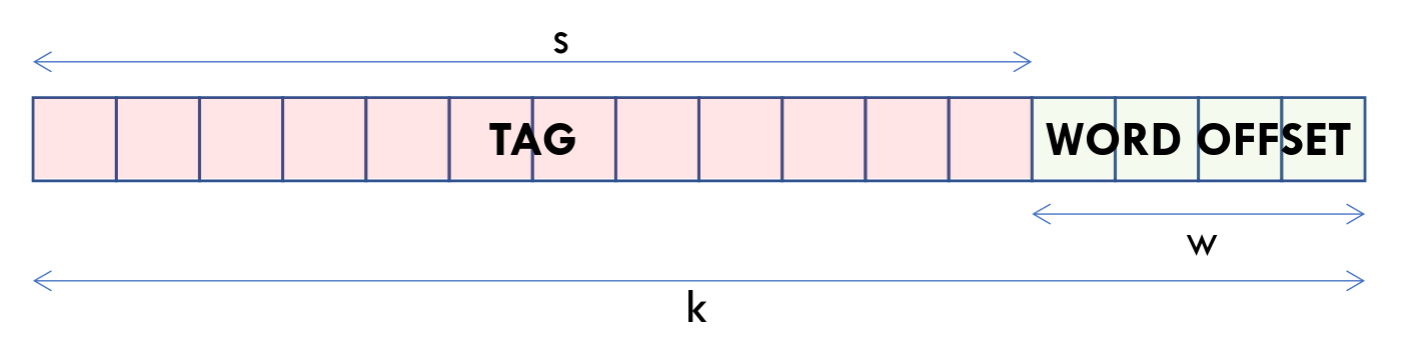
\includegraphics[scale=0.22]{../figures/cache_flassoc.png}
\end{center}

Basically, in mapping terms, we can say that TAG is the same size as \textit{Block} index, and there is no \textit{Line} index.

At this point, given the address of some data, we match the TAG with the entire CAM (only valid entries).
\begin{itemize}
	\item We first match the TAG with the CAM;
	\item On MISS, we read the memory block from DRAM at address \textit{Blockaddress}.
	Need a replacement policy if cache is full.
	After that, the block data is stored in the SRAM, in the same line as TAG.
	A validity bit is set, and we read the word at \textit{Word Offset} of the line;
\item On HIT we read the word at \textit{Word Offset} in the line that generated high when matching with the tag.
\end{itemize}

Let's talk about performance.
The advantages are the best use of the cache, and the best hit rate possible.
This means we ossibly get the best performance.

The disadvantages, of course, are the complexity to implement, the costs, and the fact that we need a large CAM with higher power dissipation and higher delays.

\subsubsection{Set associative mapping cache}

Set associative mapping is an in-between approach between direct mapping and fully associative.

Cache lines are grouped into \textbf{sets}:
\begin{itemize}
	\item \textbf{Nsets} is the number of sets;
	\item \textbf{Setlines} the number of lines in a set.
\end{itemize}
From this we have that:
$$
\text{Nsets} = \frac{\text{Nlines}}{\text{Setlines}}
$$
And the bits needed to identify a set are:
$$
d = \log_2 ( \text{Nsets} )
$$

We have \textit{direct association} of a main memory block towards a set, and \textit{fully Associative association} within that set.

\begin{center}
	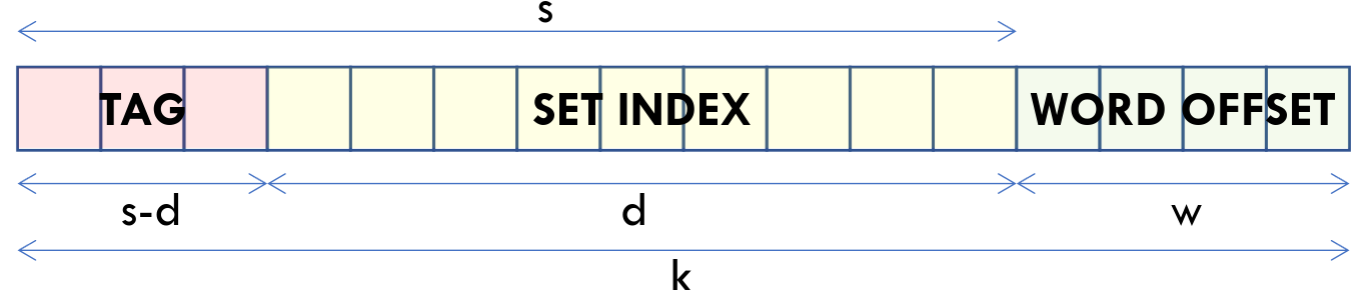
\includegraphics[scale=0.22]{../figures/cache_fac.png}
\end{center}

As with common direct mapping, the set index is $\text{Set} = \text{Blockindex} \% \text{Nsets}$, and the TAG is $(s - d)$ bits long.

At this point, fiven the address of some data, we:
\begin{itemize}
\item
Match the TAG with the CAM of the \textit{Set} pointed by the \textit{Set} index (only valid entries).
There are \textit{Nsets} separate CAMs, each of \textit{Setlines} entries;
\item
On MISS, we Read the memory block from DRAM at address \textit{Blockaddress}. The TAG is stored in the CAM of the \textit{Set}, in the next empty line.
We of course need a replacement policy if the set is full (\textbf{LRU}, \textit{Least Recently Used}, is a good candidate).
The block data is then stored in the SRAM, in the same line as TAG.
A validity bit is set for the line, and we read the word at \textit{Word Offset} in the line.
\item
On HIT, we read the word at \textit{Word Offset} in the line that generated HIT when matching.
\end{itemize}

\subsubsection{Cache replacement policies}

When a cache is full, a cache line must be replaced to store a new one.
That is our \textit{cache replacement policy}.
We have a few options:
\begin{itemize}
	\item \textbf{Direct mapping}: we have no choice, may replace a cache line even if the cache is not full;
	\item \textbf{Associative mapping}: set associative mapping may replace a cache line even if the cache is not full (but the target set is full). The algorithms are:
		\begin{itemize}
			\item \textbf{LRU} (\textit{Least Recently Used}): we store timestamps of last usages. The con is the need to sort timestamps (within a set or within the full cache, for Set and Fully associative, respectively). Intel processors used some interesting heuristics to approximate this in the 486 era;

			\item \textbf{LFU} (\textit{Least Frequently Used}) we use counters to know the number of accesses. We need to sort number of accesses (within a set or within the full cache, for Set and Fully associative, respectively);

			\item \textbf{FIFO} (\textit{First In, First Out}): we restart from first line when the bottom (of a set or the full cache) is reached. A simple pointer is required (one for each set, or one for the full cache, for Set and Fully associative, respectively);

			\item \textbf{Random} choice is not that useful, but sometimes involved in lower steps of more complex algorithms.
		\end{itemize}

\end{itemize}

\subsubsection{Cache consistency policies}

We then need policies on how we handle \textit{writes} thorugh the cache.
That is, when writing, we have decide how to update cache and main memory.
This is important especially in multi-core systems and with peripherals accessing the memory, where each core has a dedicated cache.

A few approaches:
\begin{itemize}
	\item \textbf{Write through}: all writes go to main memory as well as cache.
Multiple CPUs can monitor main memory traffic to keep local caches up to date
When a core makes a write, the other cores invalidate the cache entry relative to the written block. This involves lots of traffic, which slows down write operation.
On the other hand it has the best consistency.
Plus note that on average, only 15\% of memory references are writes.
\item \textbf{Write fatback} the update is initially made in cache only. An update bit is then set for cache line (usually called the \textit{dirty bit}).
If line is to be replaced in cache, we write back to main memory if dirty bit is set.
This saves a lot of traffic on the memory bus, and makes for improved performance.
The tradeoff is of course the fact that other caches get out of sync with the dirty ones (or in fact they might have different dirty values to write back concurrently).
\end{itemize}

\subsection{Programmable Logic Devices}

A \textbf{PLD} (\textit{Programmable Logic Device}) is a way to implement custom computation hardware for a given application.

We said (in some course, don't remember which) that there are a few approaches to computation logic design:
\begin{itemize}
	\item \textbf{Full custom IC}s: these obviously give the best performance and power consumption, but with very high NRE costs (masks, design). Designing a custom IC requires a long time-to-market, and is good only for demanding very high volume designs;
	\item \textbf{Gate array}s: these have very good performance and power, with high NRE costs (masks). We only need to build the higher layers masks, not the full IC like in full custom. Still, this has long time-to-market, and is good for high volume designs. 

		Note that, altough \textbf{FPGA}s (\textit{Field Programmable Gate Array}) have "gate array" in their name, they are usually considered PLDs.
		The good mental model is that gate arrays require additional IC routing after manufacturing, whereas PLDs are programmable after manufacturing, typically using SRAM configuration bits, flash, or antifuses;
	\item \textbf{Programmable Logic Device}s: good performance and power (compared to software), with low NRE costs (compared to a custom IC).
There are no masks involved, and the user buys an already manufactured integrated circuit.
This involves higher per-unit costs, so it's good for low volume designs and prototypes.
\end{itemize}

To summarize, a PLD is an integrated circuit (hardware device) that contains logic elements of various complexities.
The interface allows the designer to configure and connect them in different ways, configurating the device after manufacturing.
A PLD implements a hardware digital circuit, where the function of the circuit is configured by the user of the PLD.
The masks do not depend on the implemented function, so the same device can be used for different applications.
PLDs can be produced in large volumes, with NRE costs (for the PLD manufacturer) spread over many different customers.

PLDs can be configured to implement a logic circuit, either combinational or sequential.
The final circuit is hardware, not software, but it is usually described using a high level “programming” language (VHDL, Verilog, SystemC, Chisel, HLS).
Designers define internal logic functions, Interconnections and pin, using said language.

\textit{Technologies} used to configure PLDs are:
\begin{itemize}
	\item Fuse, anti-fuse (one time programmable, think OTP-ROMs, 7.1);
	\item Floating gate (reprogrammable, think EPROMs and EEPROMs, 7.2 and 7.2.5);
	\item SRAM (reprogrammable, reconfigurable at run-time, faster than floating gate technolog.
\end{itemize}

\subsubsection{ROM based PLDs}

We know from Shannon's theorem that memories (LUTs) and multiplexers can implement any combinational logic functions.
For instance, a $2^m \times n$ can implement any set of $n$ functions of $m$ shared inputs.

The memory can be OTPROM, EPROM, E2PROM (permanent), SRAM (volatile).
Definitely, it can't be ROM, otherwise we would make it full custom.
Also not NAND Flash, because of the clunky sequential read access.
Lastly, not DRAM, because of the complex access protocol (and active refreshes).

When used as a circuit, the memory is always read: it is written only before its use, to configure the circuit.

\end{document}
